\documentclass{inets-thesis}

% For editing the LaTeX environment, refer to owndefs.tex. Don't edit the inets-thesis.cls file!

% Title of the thesis
\ThesisTitle{Coexistence Study on Different Medium Access Mechanisms Using a Software Defined Radio Testbed}

% Thesis type ("M" = master thesis, "B" = bachelor thesis)
\ThesisType{B}

% Author's name (firstname(s) lastname)
\ThesisAuthor{Alexander Pastor}

% Date (year month day)
\ThesisDate{2017}{10}{24}

% Examiners: Check who is your first examiner from our professors.
% There is always one first examiner (listed in your registration sheet), and one more examiner
% who in our case is usually the respective other professor, supervisors are non-faculty members
% who supported you in addition to the first examiner in the development of the thesis
% Advisers: Reference with name and title, note that old German titles (Dipl.-Ing.) and doctor titles (Dr. or % Dr.-Ing.) are prefix while ``M.Sc.'' is a postfix to the name of the person
\FirstExaminerName{Prof.~Dr.~Petri M\"ah\"onen}
\SecondExaminerName{Prof.~Dr.-Ing.~Marina Petrova}
\SupervisorNames{Peng~Wang,~M.Sc.\\Andra~Voicu,~M.Sc.}

\begin{document}

%\chapter{First Chapter Heading}

Use\footnote{This is a footnote to the word ``use''.}
\emph{The Not So Short Introduction to \LaTeXe}~\cite{Oetiker00}
to familiarize yourself with \LaTeX. When citing research papers, use a protected space ($\sim$) in front of the \texttt{cite} command, e.g. see this reference~\cite{inproceedings}.

For tables, see \url{http://www.inf.ethz.ch/personal/markusp/teaching/guides/guide-tables.pdf} on how to design them nicely. We are also giving an example in Table~\ref{tab:example}.

Learn how to properly manage your bibliography and ensure that if you cite~\cite{Achtzehn2015,ETSI2015,FCC,Fraga-Lamas2015} you use the right types and fields. Copying BibTeX blobs from the Internet is generally not a good idea.
\section{First Section Heading}

You can simply list a number of items as
\begin{itemize}
\item Bullet Item
\item Bullet Item
\end{itemize}

\noindent You can also enumerate them as
\begin{enumerate}
\item Bullet Item 
\item Bullet Item
\end{enumerate}
\subsection{First SubSection Heading}

Use the acronym package like this: \ac{SNR} % also \acs{}, acp{}, \acf{}, acl{}
You will need to specify each acronym in the abbreviations.tex file in the appendix. For more information, see \url{http://mirrors.ctan.org/macros/latex/contrib/acronym/acronym.pdf}.

\subsubsection{First SubSubSection Heading}

Referencing of figures: Use capital notation, e.g. ``In Figure~\ref{fig:inets-logo} we show the logo of the institute.''. Same applies for tables, e.g. ``Table~\ref{tab:example} lists the parameters we used in our simulation.'' However, do not capitalize in (non-numbered) case, e.g. ``It becomes apparent from the figure that\dots'' or ``The parameters listed in the table have been selected\dots''.
\begin{figure}\begin{center}
  \includegraphics[width=\textwidth]{pictures/inets_new} % width can be fractional, e.g. width=0.45\textwidth.
  \caption{iNETS logo.}\label{fig:inets-logo}
\end{center}\end{figure}

With numbering and alignment for all equations:
\begin{eqnarray}
\lambda&=&0.25 x^0 + 0.0001\\
       &=&2.5\cdot10^{-10} x^3 + 0.0001.
\end{eqnarray}


With partial numbering for equations:
\begin{eqnarray}
\lambda&=&0.25 x^0 + 0.0001 \nonumber \\
       &=&2.5\cdot10^{-10} x^3 + 0.0001.
\end{eqnarray}

\begin{table}
\centering
 \begin{center}
\begin{tabular}{p{2.8cm}p{0.2cm}p{1cm}rp{0.2cm}p{1cm}r}
\toprule
&&\multicolumn{2}{c}{set 1}&&\multicolumn{2}{c}{set 2}\\
\cmidrule{3-4}\cmidrule{6-7}
parameter &&value&precision&&value&precision\\
\midrule
param 1 [MHz]&& 1 & $\pm$1 && 2 & $\pm$1 \\
param 2 [s]&& 1 & $\pm$0.1 && 2 & $\pm$0.2 \\
\bottomrule
 \end{tabular}\caption{Table example.} \label{tab:example}
 \end{center}

\end{table}

\unit[25]{$\mu m$} = \unit[25\,000]{nm},
\unit[0]{$^\circ \text{C}$} = \unit[273.15]{K}, and
\unit[1]{Mbit/s} = \unit[$1\,024$]{kbit/s}. Always use SI prefixes (\url{http://physics.nist.gov/cuu/Units/prefixes.html}) in text, in comparative tables use engineering notation (\url{http://www.augustatech.edu/math/molik/notation.pdf})!

 When defining symbols, make sure to put multi-letter symbols/indexes into a proper text statement, e.g.
 \begin{eqnarray}
S_\text{off} \ge S_\text{on} \\
 \text{SINR} \le \text{SNR} 
 \end{eqnarray} 
\chapter{Introduction}
\label{ch:introduction}

In this chapter we motivate the thesis and explain its structure by briefly summarizing the contents of each chapter.

Licensees of dedicated frequency bands aim at extending their bandwidth by making use of unused capacities in unlicensed bands to accommodate the growing number of users and the demand for higher transfer rates. One example is LTE Unlicensed, which aggregates carriers in the license-free 5 GHz band already populated with dual-band WLAN devices \cite{nihtilä13}\cite{qualcomm15}. However, the original LTE technology was not designed to coexist with other technologies in the same channel. Particularly, LTE in the licensed bands relies on the fact that all access to the physical medium is coordinated by a base station \cite{ghosh10}. Another unlicensed band, namely the 2.4 GHz band, is currently much more populated. IEEE 802.11 (WLAN), Bluetooth and IEEE 802.15.4 (ZigBee) devices all coexist in the 2.4 GHz band \cite{lee07}. The specifications and standards of these three technologies already offer coexistence mechanisms especially in view of rapid network densification \cite{bhushan14}. In order to facilitate harmonious coexistence of devices in the same channel the appropriate design of medium access control (MAC) protocols to avoid collisions is decisive, because collisions may render all transmitted data useless. The intention of this thesis is to examine how different MAC mechanisms and the choice of related parameters affect the performance in terms of throughput and other metrics. Our results are based on measurements with real, programmable devices making use of the flexibility of software-defined radio. In contrast to other studies \cite{gomezmiguelez16}\cite{capretti16} that have put emphasis on aspects such as transmission power, bandwidth and duty cycles of a LTE variant designed for coexistence with Wi-Fi, we focus on timing aspects of CSMA/CA, the MAC protocol used in WLAN, such as interframe spacing, backoff slot duration and contention window.

In Chapter \ref{ch:background} we discuss the theoretical foundations of the ensuing experiments. We classify and introduce a number of MAC protocols considering strengths and weaknesses of some of their mechanisms. Furthermore, we will briefly introduce the main concepts of the software tool (GNU Radio) we used for our experiments. The purpose of Chapter \ref{ch:related-work} is to put our work into the context of related work, highlighting similarities and differences in the execution of the experiments and considered MAC aspects.
In Chapter \ref{ch:methodology} we give an overview of the conducted experiments. We provide all necessary information to reproduce our results. Moreover, we define the metrics that we have taken and how our automated measurement scripts greatly reduce the required user efforts to obtain results.
Chapter \ref{ch:results} contains the measurement results and our interpretation concerning the fitness of the protocols and their mechanisms for harmonious coexistence. 
In the final chapter we discuss the main findings of Chapter \ref{ch:results} and give an outlook on possible starting points for future work.
\chapter{Background}

In this chapter the theoretical foundations and tools for the succeeding work are treated.
Firstly, the MAC layer is introduced in the context of the OSI reference model. Successively, a glance on a number of different MAC protocols and mechanisms is taken, while analyzing weaknesses with respect to the challenges coming up in wireless transmission. The chapter concludes with naming the advantages of software-defined radio.   

\bigskip

\section{MAC Protocols}

\subsection{MAC Layer in the OSI Model}

The OSI model is a layered architecture that divides a telecommunication system into several manageable layers. The original model features seven layers, where the focus in this thesis is on the MAC layer. Nevertheless, each layer's responsibilities is briefly listed. Then, a closer look on different realizations of the MAC layer is taken. Note that the data link layer has been split into two sublayers: the medium access and the logical link control sublayers.

% Sketch of ISO/OSI-model

\begin{table}[h]
	\centering
	\begin{center}
		\begin{tabular}{p{3.5cm}p{10cm}}
			\toprule
				Layer & Responsibilities \\
			\midrule
				Physical Layer & dealing with mechanical, electrical and timing interfaces of data transmission  \\
				MAC Sublayer & controlling medium access and frame synchronization \\
				LLC Sublayer & multiplexing to enable different network protocols coexist, flow control and error control.  \\
				Network Layer & routing and congestion control \\
				Transport Layer & transmission reliability, same-order-delivery, congestion avoidance  \\
				Session Layer & token management, dialog control, synchronization \\
				Presentation Layer & abstracting syntax and semantics of transmission \\
				Application Layer & user application protocols, such as http, ftp, smtp and many more \\
			\bottomrule
		\end{tabular}\caption{Layers in the OSI model} \label{tab:osi-layers}
	\end{center}
\end{table}

\subsection{ALOHA}

ALOHA is arguably the most simple MAC protocol. The basic idea is whenever a user wants to send data he does so. The higher the channel load, i.e. sending requests per time unit, the more likely collisions will occur, which render all transmitted information useless.

\bigskip

The question that comes to mind is, how likely is it that a collision will not occur. In other words, how efficient is an ALOHA channel? Making a statement requires a few preliminary assumptions:

\smallskip

\begin{enumerate}
	\item We are taking a look at pure ALOHA as described above.
	\item We simplify the calculation by assuming a fixed frame length.
	\item The number of packets generated during a frame time is a poisson-distributed random variable $X$.
	\item The channel load $G$ comprises of two portions: "new" and retransmitted frames.
\end{enumerate}

\bigskip

The probability mass function of the Poisson distribution and thus the probability of $k$ frames being generated during a given frame time amounts to:

\begin{equation}
	Pr(X=k) = \frac{G^k\cdot e^{-G}}{k!}
\end{equation}

The probability of zero frames being generated during the transmission of the frame is $Pr(X=0) = e^{-G}$ (assumption 3). If no collision occurs during the transmission of frame $F$ no other frame was sent off during that transmission. Conversely, $F$ itself did not collide with a frame sent off prior to $F$. We conclude that the vulnerability period during which collision may corrupt data is two frame times (assumption 2).

\bigskip

The probability that no frame other than the frame to be transmitted is generated during the two frame time vulnerability period is $P_0 = e^{-2G}$. The throughput $S$ is given by $S=GP_0 = Ge^{-2G}$.

\bigskip

The maximum throughput is achieved when $\frac{\partial S}{\partial G} \stackrel{!}{=} 0$:


\begin{eqnarray}
	& \frac{\partial S}{\partial G} & = \frac{\partial}{\partial G} Ge^{-2G} \\ 
	& & = e^{-2G}(1-2G) \\
	& & \stackrel{!}{=} 0 \\
	\Leftrightarrow & G & = 0.5
\end{eqnarray}
	

\bigskip

This means that for $G=0.5$ the throughput S reaches its maximum $S_\text{ALOHA,max} = \frac{1}{2e} \approx 0.18$. This result is very reasonable, since the transmission of a frame is vulnerable for the duration of two frame times, so the maximum is achieved when sending exactly every second slot, where a slot is equivalent to the frame time.

\bigskip

As an aside, the throughput can be doubled with slotted ALOHA. In contrast to pure ALOHA, slotted ALOHA allows transmission only at the beginning of slots, which effectively halves the vulnerability period to only one slot, since frames transmitted prior to a frame $F$ cannot interfere with $F$ anymore. Thus, $S_\text{ALOHA,max} = \frac{1}{e} \approx 0.36$, reached at $G=1$. However, this comes at the cost of an additional frame delay of $t_\text{slot}$ in the worst case and $\frac{t_\text{slot}}{2}$ in the average case.

\begin{figure}[h]
	\label{fig:aloha-performance}
	\begin{center}
		\includegraphics[width=13cm]{pictures/aloha_performance}
	\end{center}
	\caption{Pure ALOHA and slotted ALOHA's performance.}
\end{figure}

As shown above in figure \ref{fig:aloha-performance} and the preceding paragraphs ALOHA's performance is discouraging and improvements over ALOHA were found. 

\subsection{CSMA}

Main problem of ALOHA is the negligence of concurrent traffic in the channel. A solution to this problem is offered by the "listen before talk" (LBT) mechanism, which means in order to avoid collisions we sense the channel and refrain from sending should it be busy. This is the simple, yet effective basic idea of carrier sensing multiple access (CSMA) which comes in three flavors, as depicted in figure \ref{fig:csma-flavors} which will be discussed next.

\begin{figure}[htp] \label{fig:csma-flavors}
	\begin{center}
		\subfloat[1-persitent CSMA]{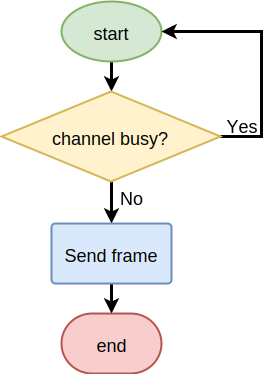
\includegraphics[width=0.22\textwidth]{pictures/csma_1_persistent}}
		\qquad
		\subfloat[non-persistent CSMA]{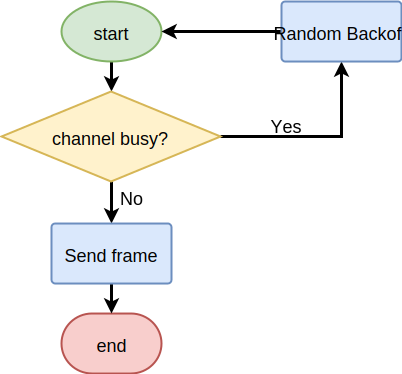
\includegraphics[width=0.31\textwidth]{pictures/csma_non_persistent}}
		\qquad
		\subfloat[p-persistent CSMA]{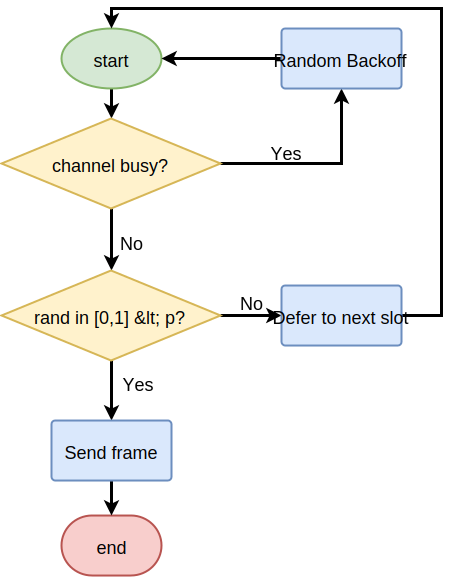
\includegraphics[width=0.35\textwidth]{pictures/csma_p_persistent}}
	\end{center}
\caption{The three flavors of CSMA}
\end{figure}


\subsubsection{1-persistent CSMA}

% 1-persistent CSMA flowchart

When the channel is busy 1-persistent CSMA waits until the channel becomes idle. As soon as the channel is found idle a frame is transmitted with a probability of 1, hence 1-persistent CSMA. If the frame collides with another, the node waits for a random backoff time and then the whole process is started all over again.

\bigskip

Despite being a substantial improvement over ALOHA, this protocol has at least two problems:

\begin{itemize}
	\item Provided propagation delay is zero or negligible, collisions can still occur.  Imagine a three-node-scenario with nodes $A$, $B$ and $C$. $A$ is transmitting, while $B$ and $C$ are waiting for their turn. Once $A$ finished transmission $B$ and $C$ will lunge onto the channel like a pack of wolves leading to collision.
	
	\item If propagation delay is not negligible the protocol suffers from another problem. In this scenario $A$ has just begun sending. $B$ will assume the channel is idle and send off his frame, since, due to the propagation delay, $B$ has not yet heard of $A$. This is why propagation delay may significantly hamper this protocol's performance.
\end{itemize}  

\subsubsection{Non-persistent CSMA}

% non-persistent CSMA flowchart 

In order to alleviate 1-persistent CSMA's problem with several nodes trying to seize the channel as soon as it becomes idle a less greedy attempt is made with non-persistent CSMA. Instead of continuously sensing the channel until it becomes idle nodes wait a random backoff time until they listen again. As a result, this protocol leads to better channel utilization with the downside of higher delays.

\subsubsection{P-persistent CSMA}

% p-persistent CSMA flowchart

P-persitent CSMA is a protocol for slotted channels. Whenever a node $A$ wishes to send off a packet the channel is sensed. If the channel is found idle it transmits its packet with a probability of $p$. With a probability $1-p$ it defers the transmissions to the next slot. This process is repeated until one either the packet is sent off or the channel is found busy again. In the latter case $A$ acts as though a collision had taken place and waits a random time until starting again.

\bigskip

This flavor of CSMA can be regarded as a compromise between 1-persistent CSMA and non-persistent CSMA, where the choice of $p$ determines the greediness. The smaller $p$, the less greedy and thus the closer p-persistent CSMA approximates non-persistent behavior. An appropriate choice of $p$ can get the best out of both worlds: minimal delays as in 1-persistent CSMA, as well as high channel efficiency as in non-persistent CSMA.

\subsection{CSMA with Collision Detection}

A way to further improve CSMA-family protocols is to immediately cancel transmissions once a collision is detected. There is no point in continuing these transmissions, as the transmitted data is lost in any case. Stating the obvious, aborting transmission saves both bandwidth and time. 

\bigskip

CSMA/CD is used on wired LANs and serves as basis of the wide-spread Ethernet. However, this mechanism is not extensively made use of in wireless networks. Concerning the reason, it is cardinal to understand that collision detection is an analog process. A collision is detected by comparing the received and transmitted signal's energy or pulse width, which premises transmission and reception taking place simultaneously. 

\bigskip

This condition mostly is not met for wireless nodes, which are half-duplex. The reason for this lies in the conservation of energy.

\begin{equation}
	P = \int_{A} I(\vec{x}) \, dA
\end{equation}

Where $P$ is the power, $I$ the intensity as function of the position $\vec{x}$ and $dA$ the differential element of a closed surface around the source. Assuming that the integration takes place over the surface of a sphere with the radius $r$ the term simplifies to:

\begin{eqnarray} 
	& P = & \abs{I(r)} \cdot 4\pi r^2 \\
	\label{eqn:intensity}
	\Leftrightarrow & \abs{I(r)} = & \frac{P}{4\pi r^2} 
\end{eqnarray}

Another, and more common quantity in telecommunications is signal-to-noise ratio (SNR), which is defined as follows, where $P$ is the signal power and $N$ the noise power: 

\begin{equation} \label{eqn:snr}
	SNR [dB] = 10 \, log \left( \frac{P}{N} \right)
\end{equation}

Equations \ref{eqn:intensity} and \ref{eqn:snr} imply if we increase the distance $r$ by $\sqrt{2}$ the signal's intensity halves or lose 3dB in SNR, respectively. To make up for the loss in signal strength we would have to employ expensive signal processing hardware making wireless equipment less affordable. Alternatively, we could increase the transmit power, but this increases interference with other nodes, as well as electricity consumption.  

\subsection{Challenges for Wireless MAC Protocols}

Wireless MAC protocols have to tackle a few problems that do not occur in wired data exchange. Among them are the hidden node and the exposed node problem, which will be discussed by reference to \ref{fig:hidden_exposed_node_problem}. Further challenges, such as energy limitations will also be delineated.

\subsubsection{The Hidden Node and the Exposed Node Problem}

\begin{figure}[ht]
	\label{fig:hidden_exposed_node_problem}
	\begin{center}
		\includegraphics[width=12cm]{pictures/hidden_exposed_node_problem}
	\end{center}
	\caption{Setup to explain the hidden and exposed node problem. Each node can only reach its neighbors.}
\end{figure}

Suppose that the node's radio range is limited to the neighboring nodes and $A$ would like to transmit to $B$. If $C$ just started transmitting $A$ won't hear $C$ and falsely assume that the channel is idle and start transmitting. This is the hidden node problem.

\bigskip

For the same configuration, in another scenario $B$ would like to send to $A$ and $C$ is already transmitting to $D$. $B$ refrains from sending despite collisions would only take place between $B$ and $C$, where it does not matter. This is the exposed node problem. 

\bigskip

\subsubsection{Further Challenges}

% Citation needed for verification
Further challenges to MAC protocol design include the power conservation when faced with constrained power resources, as in wireless sensor networks (WSN) where devices rely on batteries for their supply with power. Attempts to mitigate waste of energy have been made in several specialized, duty-cycle based MACs such as Sensor MAC, Timeout MAC and Berkley MAC.

\bigskip

On the same page, due to constrained energy resources, WSN are especially susceptible to denial of sleep attacks, a special form of denial of service (DoS) attack, drastically increasing energy consumption and thus reducing the system's lifetime. It is due to this fact that security is paramount in biomedical or military fields of application. 

\subsection{CSMA with Collision Avoidance}

802.11 is a set of physical layer (PHY) and MAC specifications for wireless local area networks (WLANs). When the dominant mode of operation, the so-called distributed coordination function (DCF) is employed CSMA/CA is used in the MAC layer.

\bigskip

Beside physical carrier sensing previously simply referred to as carrier sensing another mechanism, namely virtual carrier sensing in combination with RTS/CTS exchange is employed to mitigate the trouble caused by hidden nodes. 

\bigskip

In order to explain these mechanisms we refer to the setup of figure \ref{fig:hidden_exposed_node_problem} with a slight modification in so far as that each node's radio range shall span across two neighboring nodes in both directions. That is to say, $A$ can hear $B$ and $C$, but not $D$ and so on. Figure \ref{fig:virtual_carrier_sensing} visualizes the chain of events whose explanation follows.

\bigskip

\begin{figure}[ht]
	\label{fig:virtual_carrier_sensing}
	\begin{center}
		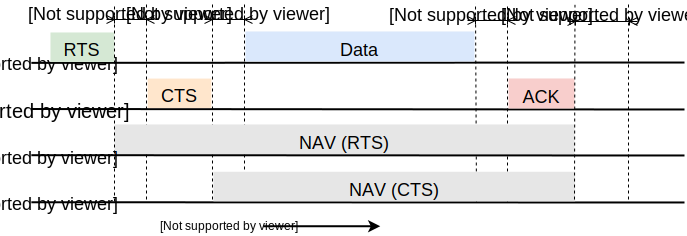
\includegraphics[width=14cm]{pictures/virtual_carrier_sensing}
	\end{center}
	\caption{Virtual Carrier Sensing in CSMA/CA}
\end{figure}

$A$ wants to send to $B$, hence issues a request to send (RTS). Every node receiving the RTS is shut down, except for $B$ that in response to the RTS creates a clear to send (CTS) frame. Not only $A$ receives this CTS frame, but also $D$, a hidden node from $A$'s point of view. Upon reception of CTS $D$ is silenced as well. Therefore, RTS/CTS is addressing the hidden node problem. RTS/CTS are frames of 30 bytes length containing the length of the frame in this case $A$ wants to transmit. Based on this length $C$ and $D$ setup the so-called network allocation vector (NAV), which are node-internal timers reminding $C$ and $D$ that the channel is still in use. Due to the fact, that no physical process is running to detect the channel status this mechanism get its name virtual carrier sensing. Shutting down nodes has the beneficial side-effect of reducing overhearing and therefore reduces energy consumption.

\bigskip

As further depicted in figure \ref{fig:virtual_carrier_sensing} there are named intervals of specified length between each of the frames. Varying lengths of these interval types serve the purpose of prioritizing certain frames over others. 

\medskip
The short interframe spacing (SIFS) is the interval until the next control frame or next fragment (of a fragmented data frame) may be sent. SIFS is designed to allow one party out of the two parties in dialog send off their frame without interference by another node. 

\medskip
The longer interval DCF interframe spacing (DIFS) is the interval after which any station may try to seize the channel for their transmission.

\medskip
For the sake of completeness, we briefly mention two consciously left out intervals, namely point coordination function interframe spacing (PIFS) and extended interframe spacing (EIFS). If 802.11 is operated in an alternative mode of operation, where a base station acts as a coordinator of traffic the standard prescribes an interval of length PIFS to allow the base station to send certain control (beacon and poll) frames. EIFS is used to report the reception of a bad or unknown frame and due to this action's low priority is the longest interval among the mentioned four. 

\bigskip

As a remark on the exposed node problem: MAC protocols such as MACA that feature the RTS/CTS exchange, but no ACK from the receiver also solve the exposed station problem. The inclusion of the ACK however "resurrects" the exposed station problem, since the receiver's ACK can now interfere with node's that are out of the sender's range. However, renouncing on ACKs was dropped in the revised version MACAW, because the absence of lost frames was not noticed until much later in the transport layer, causing huge drops in throughput.

\subsection{Duty-Cycle-Based MAC Protocols}  

... Sensor MAC, Timeout MAC, Berkley MAC ...

\section{Software Defined Radio}
 
\subsection{Purpose of Software Defined Radio}

% figure of fm/am radio electrical circuits
Traditional radio equipment is "hardware-defined", i.e. that the signal processing runs on a specialized electrical circuit.

\subsection{GNU Radio}



%\chapter{Related Work}

\section{Coexistence Study by Gomez-Miguelez et al.}

Gomez-Miguelez et al. propose srsLTE, an open-source SDR library for the PHY layer of LTE release 8 \cite{gomezmiguelez16}. In contrast to many earlier simulation-based studies they have actually set up physical devices, better reflecting system level details of both technologies and providing insight for real-world deployments \cite{rupasinghe14} \cite{nihtilä13} \cite{jeon14} \cite{cavalcante13} . Their testbed comprises of several WiFi and LTE links, for which they used Ettus USRP B210 boards (LTE) and low-power single-board computers from Soekris (WiFi). In order to detect vendor-specific performance issues they decided to use two different sets of wireless NICs from Atheros and Broadcomm.

In their study the influence of the following parameters was examined: LTE-U duty cycle, WiFi and LTE TX power, LTE bandwidth, LTE central frequency (i.e. LTE and WiFi spectrum overlap).

Their main results can be summarized as follows:

\begin{itemize}
	\item WiFi throughput is inversely proportional to LTE duty cycle.
	\item WiFi TX power has little impact on WiFi throughput.
	\item The influence of LTE bandwidth and central frequency on WiFi throughput depends very much on the vendor of the NIC card. As a result, more experimental research with physical devices from different vendors is strongly recommended. 
\end{itemize}

\section{Coexistence Study by Capretti et al.}

Another empirical study \cite{capretti16} conducted by Capretti et al. also evaluates LTE Unlicensed/WiFi coexistence based on LTE-U.  Their testbed consists of one eNB and one UE, one WiFi access point and five WiFi nodes. Their WiFi network was based on embedded PCs equipped with commodity wireless adapters. The LTE nodes were based on desktop computers with Ettus USRP B210 RF front ends running the open-source driver UHD. The software used includes srsLTE to build up a LTE release 8 compliant LTE stack, as well as GNU Radio. 

The following parameters were subject of interest: duty cycle, WiFi power settings WiFi MCS (modulation and coding scheme) and packet size. The metrics measured were satisfied load in percent, total WiFi throughput, WiFi jitter and LTE packet loss.  

Their main findings can be summarized as follows:

\begin{itemize}
	\item The duty cycle patterns are a main influence on achievable WiFi throughput. Particularly, shorter duty cycles decrease jitter, which is important for real-time applications. On the other hand longer duty cycles offer superior throughput due to reduced overhead.
	\item LTE suppresses WiFi transmissions if the TX power levels are comparable and no duty cycling is employed.
	\item If WiFi TX power is increased, WiFi load negatively impacts LTE throughput.
	\item There is no panacea strategy ensuring maximum WiFi throughput operating under different MCSs and packet sizes.
	\item LTE performance is unaffected by WiFi contention levels.
\end{itemize}

\section{Connection to Our Work}

Both studies aim at understanding under which circumstances duty-cycle-based LTE-U can coexist with WiFi in the unlicensed band by conducting experimental research with SDR (USRP) LTE and commodity WiFi devices. 

We, too, carry out experimental research and use USRPs to understand the influence of parameters used in CSMA/CA in a setup with two links each either employing ALOHA or a CSMA/CA on the overall performance. While the studies focus on the variation of power and bandwidth parameters of the transmission, we put emphasis on timing aspects.   

\chapter{Measurement Methodology}

This chapter is dedicated to answering the questions of what was measured and how results were obtained. Firstly, the measurement setup is discussed in view of the necessity to verify the recorded data. Subsequently,  the GNU Radio flowgraphs are explained. Secondly, with reference to the flowgraphs measurement metrics are formally defined.  Lastly, an overview of the semi-automatic measurement script system designed to automate, therefore accelerate the process of file system management, data processing and result plotting is given.

\section{Measurement Setup}

The setup consists of two USRP2s from Ettus Research and two USRP 2920s from National Instruments. Where the former pair is programmed as receiver and sniffer and the latter  as senders as depicted in \ref{fig:measurement-setup}. Each USRP was connected to a gigabit switch through a LAN cabel. The scripts running on the devices were launched from the institute's computer with the IP 134.130.223.151, which was remote controlled from my private laptop. Table \ref{tab:measurement-parameters} contains other necessary information to reproduce the measurement results.

\begin{figure}[tb]
	\label{fig:measurement-setup}
	\begin{center}
		\includegraphics[width=0.5\textwidth]{pictures/measurement_setup}
	\end{center}
	\caption{Photo of the measurement setup}
\end{figure}

% Measurement parameters
\begin{table}
	\label{tab:measurement-parameters}
	\begin{center}
		\begin{tabular}{p{2.5cm}p{2cm}p{2cm}p{1.5cm}p{1.5cm}p{2cm}}
			\toprule
			Function & TX Gain & RX Gain & Source Address & Dest. Address & IP Address\\
			\midrule
			Receiver 		& 4dB 	& 10dB 	& X 	& any	& 10.0.0.6\\
			Sniffer 		& 0 	& 0 	& any 	& any	& 10.0.0.10 \\
			Transmitter 1 	& 5dB 	& 0 	& Y 	& 	X 	& 10.0.0.9 \\
			Transmitter 2	& 9dB 	& 0 	& Z 	& 	X 	& 10.0.0.3 \\
			\bottomrule	
		\end{tabular}\caption{Setup parameters}
	\end{center}
\end{table}


\section{GNU Radio Flowgraphs}

%\subsection{Common Variables}
%
%Our GNU Radio pure ALOHA and non-persistent/1-persistent CSMA implementations are placed on top of a common PHY layer warranting comparability. The specific PHY layer implementation is beyond this work's scope, but a few parameters common to all flowgraphs shall be discussed nonetheless. Hereinafter, these variables and their values will not be mentioned unless they are important concerning the interpretation of results.
%
%\begin{figure}[ht]
%	\label{fig:grc-common-variables}
%	\begin{center}
%		\includegraphics[width=\textwidth]{pictures/grc_common_variables}
%	\end{center}
%\caption{Variables Common to All Flowgraphs}
%\end{figure}     

\subsection{Receiver and Sniffer}

Figure \ref{fig:grc-receiver} shows the two-way handshake receiving logic. After frame integrity is checked and type is confirmed to be data frame an acknowledgment is generated. The \texttt{frame\_probe} blocks record the times when the frames reach certain positions in the flowgraph representing the occurrence of events such as frame reception, passed or failed frame integrity check and more. Note that the address check is disabled so that the receiver may receive frames from any sender.

The sniffer consists only of a single \texttt{frame\_probe} block, which records detected power above noise level during the whole measurement. The sniffer provides valuable insight of what is actually going on in the channel from a "neutral" point of view. Neutral in the sense of:

\begin{itemize}
	\item A clear distinction between the senders can be made according to the energy levels, since the sniffer is located between the senders and transmission gains were chosen accordingly.
	\item Sensing the channel is possible during the whole measurement time, because the sniffer is never sending.
\end{itemize}

In a nutshell, the sniffer is a valuable debugging and verification tool as described in more detail in section \ref{sec:measurement-metrics}.

\begin{sidewaysfigure}[ht]
	\label{fig:grc-receiver}
	\begin{center}
		\subfloat[Receiver]{\includegraphics[width=\textwidth]{pictures/grc_receiver_flowgraph}}
		\vskip 40pt
		\subfloat[Sniffer]{\includegraphics[width=0.3\textwidth]{pictures/grc_sniffer_flowgraph}}
	\end{center}
	\caption{GRC Receiver Flowgraphs}
\end{sidewaysfigure}

\subsection{Pure ALOHA Transmitter}
The \texttt{run} block enables us to start several senders exactly at the same time, which is useful if we execute the flowgraphs manually without the automated measurement scripts. Payload is generated in the \texttt{dummy\_source} block, packed into a frame in the \texttt{framing} block and buffered in the \texttt{frame\_buffer} block. The interval between generated frames is determined by a \texttt{general\_timer} block, which we trigger either constant or exponentially distributed intervals. Self-reception is prevented by shutting down the receiver when about to send a frame through the sending block. As soon as the data packet is sent off the \texttt{timeout} block receives a copy of the data frame. If the timeout timer is reset by a recevied ACK before it runs out the next frame in the buffer is dequeued, otherwise the data is forwarded to the \texttt{resend\_check} block. If the maximum number of retransmissions, in our case 6 has not been reached a retransmission is issued, otherwise the frame is dropped without substitution.

\begin{sidewaysfigure}[h]
	\label{fig:grc-aloha-sender}
	\begin{center}
		\includegraphics[width=\textwidth]{pictures/grc_aloha_transmitter_flowgraph}
\end{center}
\caption{GRC Pure ALOHA Transmitter Flowgraph}
\end{sidewaysfigure}

\subsection{CSMA Transmitter}

The CSMA flowgraph aims at resembling 802.11 DCF and features CCA through thresholding in the \texttt{carrier\_sensing} block. Despite the fact that this block has the feature of adaptively determining an appropriate carrier sensing threshold we chose a fixed value of 0.002 power units (PU) \footnote{Power unit is a linear-scale unit read out via the UHD driver.}. This choice was made to make sure that ALOHA transmission power levels were not confused with noise during the adaptive CSMA noise floor detection period. 

DIFS and SIFS are realized through \texttt{general\_timer} blocks with the respective values. The design, as depicted, does not feature the RTS/CTS exhange.

\begin{sidewaysfigure}[h]
	\label{fig:grc-csma-sender}
	\begin{center}
		\includegraphics[width=\textwidth]{pictures/grc_csma_transmitter_flowgraph}
\end{center}
\caption{GRC CSMA Transmitter Flowgraph}
\end{sidewaysfigure}

\clearpage

\section{Measurement Metrics}
\label{sec:measurement-metrics}

All recorded metrics will be defined in this section. Furthermore, we will describe the way how they were obtained and how we verified them.

\subsection{Throughput}

\subsection{Round-Trip Time}

\subsection{Backoff Times}

\subsection{Channel Energy Level}

\subsection{Packet Durations}

\section{Measurement Script System}
\label{sec:script-system}

\begin{figure}[ht]
	\label{fig:script-system}
	\begin{center}
		\includegraphics[width=0.65\textwidth]{pictures/script_system}
	\end{center}
	\caption{The three-phase measurement script system}
\end{figure}
\chapter{Measurement Results}

In this chapter we discuss different combinations of MAC protocols employed on the two links.  We fist assess the measurement results where both senders employ the same MAC protocols. Subsequently, we will do the same for different combinations of MAC protocols 

\section{MAC Protocols}

\paragraph{Pure ALOHA}
For pure ALOHA senders we use the flowgraph as described in Section \ref{sec:aloha-sender} and shown in Figure \ref{fig:grc-aloha-sender}. 

\paragraph{CSMA/CA}
As mentioned in Section \ref{sec:csma-transmiter} we are not featuring the optional IEEE 802.11 RTS/CTS exchange, realize DIFS and SIFS with \code{general\_timers} and the backoff with the \code{backoff} blocks. We set the durations of SIFS, DIFS and BO to a scaled versions of the 

\paragraph{1-persistent CSMA}
For 1-persistent CSMA we use the same flowgraph as for CSMA/CA and set SIFS and backoff slot times to zero. In contrast to theoretical p-persistent CSMA we sense the channel for DIFS instead of a minimal number of samples. More accurately, we could describe the protocol as "1-persistent CSMA-like with fixed sensing duration", but for brevity's sake we will refer to it as 1-persistent CSMA.  
 
\paragraph{Traffic Saturation}
If not specified otherwise all transmitters are backlogged, i.e. we have saturated traffic. In that case the time between the generation of each packet is constant and well below the RTT. When we use the term \emph{unsaturated} the time between packets generated by the \code{dummy\_source} is exponentially distributed with $\frac{1}{\lambda}=200ms$. These packets are then buffered in a \code{frame\_buffer}. For single link scenarios this leads to Poisson-distributed traffic. 

\section{Same Protocol Combinations}

Throughout this section both transmitters are executing identical flowgraphs. Generally, when both links use the same MAC protocol we expect to see comparable results for any over a sufficiently longer period of time, although small variations are also expected due to statistical and hardware-related effects and inaccuracies. 

\subsection{ALOHA}
\label{sec:dbl-aloha}

For two links with saturated ALOHA traffic we expect zero aggregate throughput, since each and every package collides. Figure \ref{fig:results-aloha-dbl} \subref{fig:results-aloha-dbl-throughput} confirms this assumption. The corresponding packet loss of 100\% is depicted in Subfigure \subref{fig:results-aloha-dbl-packet-loss}. A reference value that can be read off Subfigure \subref{fig:results-aloha-dbl-throughput} is the throughput of a single saturated ALOHA link, which is about 130 kbps. This means that the combined throughput of multiple nodes in this channel with the same underlying PHY layer can never exceed 130 kbps and we can assess how well different protocols coexist and how much efficiently they make use of the channel by comparing their joint throughput to this value. Furthermore, a physical view on the channel from the sniffer's perspective is provided in Subfigure \subref{fig:results-aloha-dbl-channel-energy}. Due to the fact that the two transmissions of the senders are not completely overlapping we can see that we do not have a single sender with observed transmission energy level around 0.0011 PU, but instead two senders, where the observed energy level of the first transmitter is around 0.0006 PU, which the channel energy CDF in Subfigure \subref{fig:results-aloha-dbl-channel-energy-cdf} confirms. Note that the share of this particular energy (0.0006 PU) in the CDF is so high, because the transmission overlap does not stay constant throughout the whole measurement, but slightly varies with each repetition.
\begin{figure}[tb]
	\label{fig:results-aloha-dbl}
	\begin{center}
		\centerline{
			\subfloat[throughput]{\includegraphics[width=0.52\textwidth]{pictures/results/same_combinations/aloha/throughput_cdf}\label{fig:results-aloha-dbl-throughput}}
			\subfloat[packet loss CDF]{\includegraphics[width=0.52\textwidth]{pictures/results/same_combinations/aloha/packet_loss_cdf}\label{fig:results-aloha-dbl-packet-loss}}
		}		
		\centerline{
			\subfloat[channel energy]{\includegraphics[width=0.52\textwidth]{pictures/results/same_combinations/aloha/smoothed_channel_energy_level_4_line_chart}\label{fig:results-aloha-dbl-channel-energy}}
			\subfloat[channel energy CDF]{\includegraphics[width=0.52\textwidth]{pictures/results/same_combinations/aloha/smoothed_channel_energy_cdf}\label{fig:results-aloha-dbl-channel-energy-cdf}}
		}		
	\end{center}
	\caption{Measurement results for two ALOHA senders in the same channel}
\end{figure}



\subsection{CSMA/CA With High Parameter Set}

\begin{figure}[tb]
	\label{fig:results-csma-high-dbl-1}
	\begin{center}
		\centerline{
			\subfloat[throughput]{\includegraphics[width=0.5\textwidth]{pictures/results/same_combinations/csma_high_params/throughput_cdf}\label{fig:results-csma-high-dbl-throughput}}
			\subfloat[frame delay]{\includegraphics[width=0.5\textwidth]{pictures/results/same_combinations/csma_high_params/frame_delay_boxplot}\label{fig:results-csma-high-dbl-frame-delay}}
		}	
	\end{center}
	\caption{Measurement results for the CSMA/CA with high parameter set}
\end{figure}

\begin{figure}[b]
	\label{fig:results-csma-high-dbl-2}
	\begin{center}
		\centerline{
			\subfloat[channel energy CDF]{\includegraphics[width=0.5\textwidth]{pictures/results/same_combinations/csma_high_params/smoothed_channel_energy_cdf}\label{fig:results-csma-high-dbl-channel-energy}}
			\subfloat[channel energy]{\includegraphics[width=0.5\textwidth]{pictures/results/same_combinations/csma_high_params/smoothed_channel_energy_level_4_line_chart}\label{fig:results-csma-high-dbl-channel-energy-cdf}}
		}	
	\end{center}
	\caption{Energy in the channel detected by the sniffer for CSMA/CA with high parameter set.}
\end{figure}


\begin{figure}[tb]
	\label{fig:results-csma-high-dbl-3}
	\begin{center}
		\centerline{
			\subfloat[total backoff]{\includegraphics[width=0.5\textwidth]{pictures/results/same_combinations/csma_high_params/backoff_(joint)_sum_cdf}\label{fig:results-csma-high-dbl-backoff}}
			\subfloat[logical channel occupation]{\includegraphics[width=0.5\textwidth]{pictures/results/same_combinations/csma_high_params/zoomed_channel_occupation_gantt_chart}\label{fig:results-csma-high-dbl-channel-occupation}}
		}		
	\end{center}
	\caption{Measurement results for the CSMA/CA with high parameter set}
\end{figure}

First of all with "high parameter set" we mean we chose high values for DIFS, SIFS and backoff slot time (BO) from which we expected that they lead to good coexistence of the two links. In particular, we chose DIFS=15ms, SIFS=3ms and BO=6ms. Figure \ref{fig:results-csma-high-dbl-1} \subref{fig:results-csma-high-dbl-throughput} shows that the throughput roughly halves when two links are active at the same time. Subfigure \subref{fig:results-csma-high-dbl-frame-delay} shows that the frame delay roughly stays the same, where the deviation of the first link comes from packet loss related to hardware problems as described in Section \ref{sec:quality-standards}. Figure \ref{fig:results-csma-high-dbl-2} illustrates the same from the sniffer's point of view (POV), as the even throughput among senders is reflected in Subfigure \subref{fig:results-csma-high-dbl-channel-energy-cdf} with the two observed energy levels of the senders being 0.0004 PU and 0.0007 PU, which is confirmed by Subfigure \subref{fig:results-csma-high-dbl-channel-energy}. Figure \ref{fig:results-csma-high-dbl-3} shows the cumulative backoff times and the logical channel occupation which corresponds to the channel energy plot in Figure \ref{fig:results-csma-high-dbl-2} \subref{fig:results-csma-high-dbl-channel-energy}. 

\subsection{CSMA/CA With Low Parameter Set}
\label{sec:csma-dbl-low}

\begin{figure}[b]
	\label{fig:results-csma-low-dbl-1}
	\begin{center}
		\centerline{
			\subfloat[throughput]{\includegraphics[width=0.5\textwidth]{pictures/results/same_combinations/csma_low_params/throughput_cdf}\label{fig:results-csma-low-dbl-throughput}}
			\subfloat[frame delay]{\includegraphics[width=0.5\textwidth]{pictures/results/same_combinations/csma_low_params/frame_delay_boxplot}\label{fig:results-csma-low-dbl-frame-delay}}
		}	
	\end{center}
	\caption{Measurement results for the CSMA/CA with low parameter set}
\end{figure}

The next thing we were interested in is to what extent we can scale down DIFS, SIFS and BO and still retain collision-free transmission. To this end, we reduced the values to DIFS=5ms, SIFS=1ms, BO=2ms. Reducing these values, especially BO increases the throughput, with $CW_\text{min} = 32 \cdot BO$ and uniformly distributed random choice of the backoff slot, we expect a mean delay of $16\cdot BO=32ms$ in the first backoff round, which is rather large compared to DIFS and SIFS.

 Indeed, comparing throughput using the high parameter set (Figure \ref{fig:results-csma-high-dbl-1}\subref{fig:results-csma-high-dbl-throughput}) with the low parameter set (Figure \ref{fig:results-csma-low-dbl-1}\subref{fig:results-csma-high-dbl-throughput}) yields a little less than doubled throughput for cutting the backoff. 
 A problem are collisions of ACKs and consecutive data frames of the sender to whom the ACK was not destined caused by the low DIFS in conjunction with hardware delays. Multiple of these collisions occur in the time window depicted in Figure \ref{fig:results-csma-low-dbl-2}\subref{fig:results-csma-low-dbl-channel-energy}. These collisions lead to the increased frame delays of Figure \ref{fig:results-csma-low-dbl-1}\subref{fig:results-csma-low-dbl-frame-delay}, where again the additional packet loss of link 1 reflected in the 20ms increased frame delay compared to link 1 is caused by the hardware problems described in Section \ref{sec:quality-standards}.

\begin{figure}[bt]
	\label{fig:results-csma-low-dbl-2}
	\begin{center}
		\centerline{
			\subfloat[channel energy CDF]{\includegraphics[width=0.5\textwidth]{pictures/results/same_combinations/csma_low_params/smoothed_channel_energy_cdf}\label{fig:results-csma-low-dbl-channel-energy-cdf}}
			\subfloat[channel energy]{\includegraphics[width=0.5\textwidth]{pictures/results/same_combinations/csma_low_params/smoothed_channel_energy_level_4_line_chart}\label{fig:results-csma-low-dbl-channel-energy}}
		}
		\centerline{
			\subfloat[total backoff]{\includegraphics[width=0.5\textwidth]{pictures/results/same_combinations/csma_low_params/backoff_(joint)_sum_cdf}\label{fig:results-csma-low-dbl-backoff}}
			\subfloat[logical channel occupation]{\includegraphics[width=0.5\textwidth]{pictures/results/same_combinations/csma_low_params/zoomed_channel_occupation_gantt_chart}\label{fig:results-csma-low-dbl-channel-occupation}}
		}		
	\end{center}
	\caption{Measurement results for the CSMA/CA with low parameter set}
\end{figure}



\subsection{CSMA/CA With Medium Parameter Set}

\begin{figure}[tb]
	\label{fig:results-csma-med-dbl}
	\begin{center}
		\centerline{
			\subfloat[throughput]{\includegraphics[width=0.5\textwidth]{pictures/results/same_combinations/csma_med_params/throughput_cdf}}
			\subfloat[frame delay]{\includegraphics[width=0.5\textwidth]{pictures/results/same_combinations/csma_med_params/frame_delay_boxplot}\label{fig:results-csma-med-dbl-frame-delay}}
		}
		\centerline{
			\subfloat[channel energy]{\includegraphics[width=0.5\textwidth]{pictures/results/same_combinations/csma_med_params/smoothed_channel_energy_level_4_line_chart}}
			\subfloat[channel energy CDF]{\includegraphics[width=0.5\textwidth]{pictures/results/same_combinations/csma_med_params/smoothed_channel_energy_cdf}}
		}
		\centerline{
			\subfloat[logical channel occupation]{\includegraphics[width=0.5\textwidth]{pictures/results/same_combinations/csma_med_params/zoomed_channel_occupation_gantt_chart}}
			\subfloat[total backoff]{\includegraphics[width=0.5\textwidth]{pictures/results/same_combinations/csma_med_params/backoff_(joint)_sum_cdf}}
		}		
	\end{center}
	\caption{Measurement results for the CSMA/CA with medium parameter set}
\end{figure}

Due to the collisions of ACKs with the data packets of sender 1 as described in the preceding Section \ref{sec:csma-dbl-low} we increased DIFS to 9 ms, kept SIFS to 1 ms and BO to 2ms and indeed, as shown in Figure \ref{fig:results-csma-med-dbl}\subref{fig:results-csma-med-dbl-frame-delay} the frame delay of link 2 is close to the baseline level as result of avoiding collisions. However, since collisions as a result of low DIFS occurred quite infrequently in the last scenario, the metrics roughly stay the same as in the previous scenario, as can be seen in all other subfigures.

\clearpage

\subsection{1-persistent CSMA}

\begin{figure}[tb]
	\label{fig:results-difs-only-dbl-1}
	\begin{center}
		\centerline{
			\subfloat[channel energy]{\includegraphics[width=0.5\textwidth]{pictures/results/same_combinations/difs_only/smoothed_channel_energy_level_4_line_chart}\label{fig:results-difs-only-dbl-channel-energy}}
			\subfloat[channel energy CDF]{\includegraphics[width=0.5\textwidth]{pictures/results/same_combinations/difs_only/smoothed_channel_energy_cdf}\label{fig:results-difs-only-dbl-channel-energy-cdf}}
		}
		\centerline{
			\subfloat[logical channel occupation]{\includegraphics[width=0.5\textwidth]{pictures/results/same_combinations/difs_only/zoomed_channel_occupation_gantt_chart}\label{fig:results-difs-only-dbl-channel-occupation}}
			\subfloat[packet loss]{\includegraphics[width=0.5\textwidth]{pictures/results/same_combinations/difs_only/packet_loss_boxplot}\label{fig:results-difs-only-dbl-packet-loss}}
		}		
	\end{center}
	\caption{Measurement results for 1-persistent CSMA}
\end{figure}

In the following experiment we examined if a fixed sensing duration of DIFS is enough for harmonious coexistence. As can be seen in Figure \ref{fig:results-difs-only-dbl-1}\subref{fig:results-difs-only-dbl-channel-occupation} we encounter the problem described in Section \ref{sec:csma-1-persistent}, namely that both\footnote{actually three, since the receiver is transmitting ACKs} senders try to seize the channel at the same time once a sender finished their transmission. If the time granularity of the system was finer, that is to say its timing accuracy was even higher none of the nodes would start to transmit slightly earlier, leading to even further deteriorated throughput than in Figure \ref{fig:results-difs-only-dbl-2}\subref{fig:results-difs-only-dbl-throughput}. The higher packet loss (Figure \ref{fig:results-difs-only-dbl-1}\subref{fig:results-difs-only-dbl-packet-loss}) and thus higher frame delay (Figure \ref{fig:results-difs-only-dbl-2}\subref{fig:results-difs-only-dbl-frame-delay}) of link 1 compared to link 2  can be elucidated by the fact that the signal-to-interference-plus-noise ratio (SINR) ratio of sender 2 is bigger than the SINR of sender 1\footnote{Also, the SINR of the receiver's ACK signal is higher than all others.} as can be surmised from Figure \ref{fig:results-difs-only-dbl-1}\subref{fig:results-difs-only-dbl-channel-energy}. The extra bend in the channel energy CDF (Figure \ref{fig:results-difs-only-dbl-1}\subref{fig:results-difs-only-dbl-channel-energy-cdf}) roughly from 0.0006 to 0.0007 PU is a consequence of the interference which is also very visible in Figure \ref{fig:results-difs-only-dbl-1}\subref{fig:results-difs-only-dbl-channel-energy}.

\begin{figure}[tb]
	\label{fig:results-difs-only-dbl-2}
	\begin{center}
		\centerline{
			\subfloat[throughput]{\includegraphics[width=0.5\textwidth]{pictures/results/same_combinations/difs_only/throughput_cdf}\label{fig:results-difs-only-dbl-throughput}}
			\subfloat[frame delay]{\includegraphics[width=0.5\textwidth]{pictures/results/same_combinations/difs_only/frame_delay_cdf}\label{fig:results-difs-only-dbl-frame-delay}}
		}	
	\end{center}
	\caption{Measurement results for 1-persistent CSMA}
\end{figure}

\clearpage

\section{Different Protocol Combinations}

\subsection{ALOHA and CSMA/CA}
\label{sec:aloha-csma}

In this experiment we aimed at an experimental confirmation that saturated ALOHA traffic would cause CSMA/CA to stay silent during the whole measurement time. This result is confirmed by every plot in Figure \ref{fig:results-aloha-csma}. The throughput and frame delay\footnote{since no frame has ever been sent by the CSMA/CA node} (Subfigures \subref{fig:results-aloha-csma-throughput} and \subref{fig:results-aloha-csma-frame-delay}) of CSMA/CA are zero, whereas for saturated ALOHA node throughput and frame delay almost perfectly match the baseline values. The channel energy plots in Subfigures \subref{fig:results-aloha-csma-channel-energy} and \subref{fig:results-aloha-csma-channel-energy-cdf} show that only link 1 and the receiver are transmitting during a time window of 2 seconds, which also is generally true for the whole measurement duration. 

\begin{figure}[tb]
	\label{fig:results-aloha-csma}
	\begin{center}
		\centerline{
			\subfloat[throughput]{\includegraphics[width=0.5\textwidth]{pictures/results/different_combinations/aloha_csma/throughput_cdf}\label{fig:results-aloha-csma-throughput}}
			\subfloat[frame delay]{\includegraphics[width=0.5\textwidth]{pictures/results/different_combinations/aloha_csma/frame_delay_boxplot}\label{fig:results-aloha-csma-frame-delay}}
		}
		\centerline{
			\subfloat[channel energy]{\includegraphics[width=0.5\textwidth]{pictures/results/different_combinations/aloha_csma/smoothed_channel_energy_level_4_line_chart}\label{fig:results-aloha-csma-channel-energy}}
			\subfloat[channel energy CDF]{\includegraphics[width=0.5\textwidth]{pictures/results/different_combinations/aloha_csma/smoothed_channel_energy_cdf}\label{fig:results-aloha-csma-channel-energy-cdf}}
		}	
	\end{center}
	\caption{Measurement results for saturated ALOHA and CSMA/CA (medium parameter set) simultaneously active in the same channel}
\end{figure}

\clearpage

\subsection{Unsaturated ALOHA and CSMA/CA}
\label{sec:unsat-aloha-csma}

\begin{figure}[tb]
	\label{fig:results-unsat-aloha-csma-2}
	\begin{center}
		\centerline{
			\subfloat[throughput]{\includegraphics[width=0.5\textwidth]{pictures/results/different_combinations/aloha_unsat_csma/throughput_cdf}\label{fig:results-unsat-aloha-csma-throughput}}
			\subfloat[frame delay]{\includegraphics[width=0.5\textwidth]{pictures/results/different_combinations/aloha_unsat_csma/frame_delay_cdf}\label{fig:results-unsat-aloha-csma-frame-delay}}
		}	
	\end{center}
	\caption{Measurement results for unsaturated ALOHA combined with saturated CSMA/CA (high parameter set)}
\end{figure}

The next experiment tries to give a feeling, whether relatively low load unsaturated\footnote{we still refer to exponentially distributed time between each packet with $\frac{1}{\lambda}=200ms$, which gives us roughly $G_\text{ALOHA,unsat} \approx \frac{38 \text{kbps}}{130 \text{kbps}}\approx 0.3$, where 38 kbps is the baseline throughput of unsaturated ALOHA and 130 kbps the baseline throughput of saturated ALOHA. We can use this approximation, because the offered channel load of ALOHA is independent from other transmitters and saturated ALOHA approximatively consumes the whole channel capacity.} ALOHA can coexist with CSMA/CA. The throughput of the CSMA/CA sender is reduced to $\frac{18}{45}=40\%$ of the baseline value as depicted in Figure \ref{fig:results-unsat-aloha-csma-2} \subref{fig:results-unsat-aloha-csma-throughput}, while the ALOHA throughput approximately remains the same.

Only if the CSMA/CA node transmits a frame before the ALOHA node a collision can occur, which happens during seconds 8-10 of the measurement as shown in \ref{fig:results-unsat-aloha-csma-1}\subref{fig:results-unsat-aloha-csma-channel-occupation} from a logical POV or in  \ref{fig:results-unsat-aloha-csma-1}\subref{fig:results-unsat-aloha-csma-channel-energy} from a physical POV. With that in mind, we can explain why the frame delay of CSMA/CA varies much more than the frame delay of ALOHA (Figure  \ref{fig:results-unsat-aloha-csma-2}\subref{fig:results-unsat-aloha-csma-frame-delay}). The number of ALOHA packets generated during data frame transmission time (or any other period of time) is Poisson-distributed and thus the number of collisions, whereas the likelihood of collision from the POV of an ALOHA frame is dependent on the backoff which in our case is uniformly distributed. The same explanation also applies for the differing variances in packet loss as depicted in \ref{fig:results-unsat-aloha-csma-1}\subref{fig:results-unsat-aloha-csma-packet-loss}, whereas the differing values are because ALOHA recklessly pushes its packets into channel, while CSMA does not interfere with ALOHA packets when it senses energy in the channel.

\begin{figure}[tb]
	\label{fig:results-unsat-aloha-csma-1}
	\begin{center}
		\centerline{
			\subfloat[channel energy]{\includegraphics[width=0.5\textwidth]{pictures/results/different_combinations/aloha_unsat_csma/smoothed_channel_energy_level_4_line_chart}\label{fig:results-unsat-aloha-csma-channel-energy}}
			\subfloat[channel energy CDF]{\includegraphics[width=0.5\textwidth]{pictures/results/different_combinations/aloha_unsat_csma/smoothed_channel_energy_cdf}\label{fig:results-unsat-aloha-csma-channel-energy-cdf}}
		}
		\centerline{
			\subfloat[logical channel occupation]{\includegraphics[width=0.5\textwidth]{pictures/results/different_combinations/aloha_unsat_csma/zoomed_channel_occupation_gantt_chart}\label{fig:results-unsat-aloha-csma-channel-occupation}}
			\subfloat[packet loss]{\includegraphics[width=0.5\textwidth]{pictures/results/different_combinations/aloha_unsat_csma/packet_loss_boxplot}\label{fig:results-unsat-aloha-csma-packet-loss}}
		}		
	\end{center}
	\caption{Measurement results for unsaturated ALOHA combined with saturated CSMA/CA (high parameter set)}
\end{figure}



\clearpage

\subsection{Inhomogeneous CSMA/CA}


\begin{figure}[tb]
	\label{fig:results-csma-15-5-2}
	\begin{center}
		\centerline{
			\subfloat[throughput]{\includegraphics[width=0.5\textwidth]{pictures/results/different_combinations/csma_inhomogeneous/15_5/throughput_cdf}\label{fig:results-csma-15-5-throughput}}
			\subfloat[frame delay]{\includegraphics[width=0.5\textwidth]{pictures/results/different_combinations/csma_inhomogeneous/15_5/frame_delay_boxplot}\label{fig:results-csma-15-5-frame-delay}}
		}	
	\end{center}
	\caption{Measurement results for an inhomogeneous combination of CSMA protocols.}
\end{figure}

The goal of our next experiment is to examine how CSMA/CA with different parameter sets behave in the same channel. Link 1 uses the low parameter set, whereas link 2 uses the high parameter set. The throughput of link 2 as depicted in Figure \ref{fig:results-csma-15-5-2}\subref{fig:results-csma-15-5-throughput} drops to one seventh of the baseline, whereas it only drops by 20\% for link 1. The reason for this is that with reduced DIFS and BO the chance to grab the channel increases as is shown in Figures \ref{fig:results-csma-15-5-1}\subref{fig:results-csma-15-5-channel-energy}\subref{fig:results-csma-15-5-channel-energy-cdf}\subref{fig:results-csma-15-5-channel-occupation}. The frame delay increases only marginally as shown in Figure \ref{fig:results-csma-15-5-2}\subref{fig:results-csma-15-5-frame-delay}, which is due to the packet loss depicted in \ref{fig:results-csma-15-5-1}\subref{fig:results-csma-15-5-packet-loss}. The mean packet loss is for link 2 is a little below the expected value of about 1.2\%, where as for link 1 it is above that value, which is because the SINR of link 2 is higher than for link 1. The expected packet loss comprises of two components. The first component is the baseline packet loss for this measurement, which is around 0.2\%. The second component is the chance that both senders choose the same time to transmit their packet when they sensed the channel idle, which amounts to $ \frac{1}{CW_\text{min}} \cdot \frac{\text{BO}_1}{\text{BO}_2} = \frac{1}{96} \approx 1.2\% $. An idea to reduce the chance of collisions due to this phenomenon is to configure the links to have backoff slots durations that are mutually prime, i.e. have no common divisor, which probably only works if the duration of a backoff slot is big compared to the time granularity of the whole system. 

\begin{figure}[bt]
	\label{fig:results-csma-15-5-1}
	\begin{center}
		\centerline{
			\subfloat[channel energy]{\includegraphics[width=0.5\textwidth]{pictures/results/different_combinations/csma_inhomogeneous/15_5/smoothed_channel_energy_level_4_line_chart}\label{fig:results-csma-15-5-channel-energy}}
			\subfloat[channel energy CDF]{\includegraphics[width=0.5\textwidth]{pictures/results/different_combinations/csma_inhomogeneous/15_5/smoothed_channel_energy_cdf}\label{fig:results-csma-15-5-channel-energy-cdf}}
		}
		\centerline{
			\subfloat[logical channel occupation]{\includegraphics[width=0.5\textwidth]{pictures/results/different_combinations/csma_inhomogeneous/15_5/zoomed_channel_occupation_gantt_chart}\label{fig:results-csma-15-5-channel-occupation}}
			\subfloat[packet loss]{\includegraphics[width=0.5\textwidth]{pictures/results/different_combinations/csma_inhomogeneous/15_5/packet_loss_boxplot}\label{fig:results-csma-15-5-packet-loss}}
		}		
	\end{center}
	\caption{Measurement results for an inhomogeneous combination of CSMA protocols.}
\end{figure}

\clearpage

\subsection{1-persistent CSMA and unsaturated ALOHA}

\begin{figure}[tb]
	\label{fig:results-difs-only-aloha-2}
	\begin{center}
		\centerline{
			\subfloat[throughput]{\includegraphics[width=0.5\textwidth]{pictures/results/different_combinations/difs_only_aloha/throughput_cdf}\label{fig:results-difs-only-aloha-throughput}}
			\subfloat[frame delay]{\includegraphics[width=0.5\textwidth]{pictures/results/different_combinations/difs_only_aloha/frame_delay_boxplot}\label{fig:results-difs-only-aloha-frame-delay}}
		}	
	\end{center}
	\caption{Measurement results for unsaturated ALOHA combined with 1-persistent CSMA}
\end{figure}

It would not make much sense to have a second link in a channel if there already is another link that sends saturated ALOHA traffic through the channel as shown in Sections \ref{sec:dbl-aloha} and \ref{sec:aloha-csma}. For this reason link 1 uses 1-persistent CSMA and link 2 \emph{unsaturated} ALOHA. In the given scenario it does not make much sense for the CSMA/CA transmitter to back off when the channel is sensed busy either, due to fact that the ALOHA node does not use the LBT mechanism, thus "giving it the chance to transmit" is waste of time as it transmits whenever it wants anyway. Thus, removing the backoff in CSMA/CA promises higher throughput. For this reason we now compare this experiment with the one in Section \ref{sec:unsat-aloha-csma}. The assumption of increased throughput is correct as the comparison between Figures \ref{fig:results-difs-only-aloha-2}\subref{fig:results-difs-only-aloha-throughput} and \ref{fig:results-unsat-aloha-csma-2}\subref{fig:results-aloha-csma-throughput} confirms that removing backoff more than doubles CSMA throughput. It would however, make sense to back off after the reception of an ACK to give the ALOHA node a chance to send a packet. The lack of this backoff explains the increased ALOHA mean packet loss ($\approx 34\%$ total, $\approx 300\%$ increase;  Figure \ref{fig:results-difs-only-aloha-1}\subref{fig:results-difs-only-aloha-packet-loss}), which is still comparatively low due to the high SINR of the ALOHA node. A representative excerpt of the logical channel occupation is given in Figure \ref{fig:results-difs-only-aloha-1}\subref{fig:results-difs-only-aloha-channel-occupation}, where only a single ALOHA frame around second 8.8 does not collide with a CSMA packet. The energy plot in Figure  \ref{fig:results-difs-only-aloha-1}\subref{fig:results-difs-only-aloha-channel-energy} offers a more detailed physical view the channel, where the peak energy level of colliding data packets is not much higher than the energy level of a successful ALOHA transmission. In conjunction with the energy CDF in Figure \ref{fig:results-difs-only-aloha-1}\subref{fig:results-difs-only-aloha-channel-energy-cdf}, which is taking the whole measurement duration into account and has only a small bend around 0.0006 PU we conclude that if we decrease the TX power of the ALOHA node or use a less robust MCS, such as 64-QAM, ALOHA packet loss would drastically increase. 

\begin{figure}[bt]
	\label{fig:results-difs-only-aloha-1}
	\begin{center}
		\centerline{
			\subfloat[channel energy]{\includegraphics[width=0.5\textwidth]{pictures/results/different_combinations/difs_only_aloha/smoothed_channel_energy_level_4_line_chart}\label{fig:results-difs-only-aloha-channel-energy}}
			\subfloat[channel energy CDF]{\includegraphics[width=0.5\textwidth]{pictures/results/different_combinations/difs_only_aloha/smoothed_channel_energy_cdf}\label{fig:results-difs-only-aloha-channel-energy-cdf}}
		}
		\centerline{
			\subfloat[logical channel occupation]{\includegraphics[width=0.5\textwidth]{pictures/results/different_combinations/difs_only_aloha/zoomed_channel_occupation_gantt_chart}\label{fig:results-difs-only-aloha-channel-occupation}}
			\subfloat[packet loss]{\includegraphics[width=0.5\textwidth]{pictures/results/different_combinations/difs_only_aloha/packet_loss_boxplot}\label{fig:results-difs-only-aloha-packet-loss}}
		}		
	\end{center}
	\caption{Measurement results for unsaturated ALOHA combined with 1-persistent CSMA}
\end{figure}

\clearpage



\subsection{1-persistent CSMA and CSMA/CA}

In our last experiment we show that the greedy 1-persistent CSMA approach starves other CSMA/CA links. From the perspective of a CSMA/CA sender it does not matter, whether it shares a channel with a saturated 1-persistent CSMA sender or saturated ALOHA sender (Section \ref{sec:aloha-csma}). We can virtually identify no difference in the metrics (Figures \ref{fig:results-difs-only-csma}\subref{fig:results-difs-only-csma-frame-delay}\subref{fig:results-difs-only-csma-channel-energy}\subref{fig:results-difs-only-csma-channel-energy-cdf} comapared to the corresponding ones in Figures \ref{fig:results-aloha-csma}) between those combinations except for the reduced throughput \ref{fig:results-difs-only-csma}\subref{fig:results-difs-only-csma-channel-energy-cdf} due to the addition of channel sensing with the duration of DIFS compared to ALOHA. Only if we decreased the offered load of 1-persistent CSMA we could see any and better coexistence\footnote{compared to ALOHA due to the LBT mechanism that stops the 1-persistent CSMA sender from interfering with ongoing transmissions} with CSMA/CA at all.

\begin{figure}[tb]
	\label{fig:results-difs-only-csma}
	\begin{center}
		\centerline{
			\subfloat[throughput]{\includegraphics[width=0.5\textwidth]{pictures/results/different_combinations/difs_only_csma/throughput_cdf}\label{fig:results-difs-only-csma-throughput}}
			\subfloat[frame delay]{\includegraphics[width=0.5\textwidth]{pictures/results/different_combinations/difs_only_csma/frame_delay_boxplot}\label{fig:results-difs-only-csma-frame-delay}}
		}
		\centerline{
			\subfloat[channel energy]{\includegraphics[width=0.5\textwidth]{pictures/results/different_combinations/difs_only_csma/smoothed_channel_energy_level_4_line_chart}\label{fig:results-difs-only-csma-channel-energy}}
			\subfloat[channel energy CDF]{\includegraphics[width=0.5\textwidth]{pictures/results/different_combinations/difs_only_csma/smoothed_channel_energy_cdf}\label{fig:results-difs-only-csma-channel-energy-cdf}}
		}	
	\end{center}
	\caption{Measurement results for the CSMA/CA with large parameter set}
\end{figure}
\chapter{Conclusions and Future Work}

Conclusions and Future Work here.

\appendix
\chapter{Bash and Python Scripts}

This appendix aims at giving in-depth insight in the scripts used in the three phases of the measuring, data processing and plotting process. The basic principle, however, is depicted in section \ref{sec:script-system}. Minor edits were made for format and aesthetic reasons.

\begin{lstlisting}[language=Bash,caption=measure.sh]
echo "remote_measurement is set to "$remote_measurement"."

function setup_remote_connection
{
  reset
  sshpass -p "inets" ssh -$remote_flags $remote_user@$remote_ip "bash -s" < remote_measurement_$link.sh
}

function prepare_measurement
{
    reset
    measurement_counter=0
    ## let's make sure all the directories exist
    printf "\nchecking if paths exists...\n"

    #let's first make absolutely sure the raw data source path exists
    if [ ! -d $raw_data_source_path ];
      then
        mkdir -p $raw_data_source_path
        echo $raw_data_source_path" created."
      else
        rm -r $raw_data_source_path/*
    fi

    if [ -d $plot_directory_path ];
      then
        echo $plot_directory_path" already existed!"
        cd $plot_directory_path
        # create measurement directory
        while [ -d $measurement_counter ]; do
            measurement_counter=$(($measurement_counter+1))
        done
        export measurement_counter;
    fi

    if [ -d $log_path ];
      then
        echo $log_path" already existed!"
      else
        mkdir -p $log_path
        echo $log_path" directory created."
    fi

    mkdir -p $plot_directory_path/$measurement_counter
    echo $plot_directory_path/$measurement_counter" directory created."

    mkdir -p $data_source_path/$measurement_counter
    echo $data_source_path/$measurement_counter" directory created."

    mkdir -p $jobs_open_path
    mkdir -p $jobs_done_path

    ## let's check if measurement script is defined
    # if $measurement_scripts undefined:
    # go through directory and list all python files
    if [ -z ${measurement_scripts+x} ];
      then
        echo  "no measurement scripts set,
              going through files inside of $locate_base_path."
        echo "please add a the full path of one of the files to \$scritps."
        #locate -r "$locate_base_path" | grep "\.py$"
        echo "terminated. ding dong"
        exit -1
    fi

    printf "\n"
}

function measure
{
  local prematurely_aborted=0

  for ((x = 1 ; x <= $measurement_repetitions ; x += 1)); do

    # get pid to later kill it
    for i in "${measurement_scripts[@]}"
    do
      python $measurement_script_path/$i &
    done

    for ((y = $timer ; y > 0 ; y -= 1)); do
      echo "measurement $x/$measurement_repetitions complete in $y second(s)."
      if [ $check_if_prematurely_aborted -eq 1 ];
        then
          if $(ps -p ${measurement_scripts_pid[*]}) | grep ${measurement_scripts_pid[*]};
            then
              :
            else
              prematurely_aborted=1
              echo  "Scripts were killed prematurely. Measurement may be incomplete."
              break
          fi
      fi
      sleep 1
    done

    kill $(jobs -p)

    # save this measurement's data to special folder
    mkdir -p $data_source_path/$measurement_counter/$x
    echo  "measurement $x raw data directory created $data_source_path/$measurement_counter/$x/."

    echo $raw_data_source_path
    echo $(ls $raw_data_source_path | egrep "*_$link.txt")

    cd $raw_data_source_path
    mv -v $(ls | egrep "*_$link.txt") $data_source_path/$measurement_counter/$x/
    cp -v $(ls | egrep "sniffer") $data_source_path/$measurement_counter/$x/
    if [ "$receiver_mode" == "single" ];
      then
        cp -v $(ls | egrep "receiver") $data_source_path/$measurement_counter/$x/
    fi
    echo  "measurement $x raw data moved to $data_source_path/$measurement_counter/$x/."
    printf "\n"
    if [ $prematurely_aborted -eq 1 ];
      then
        if [ $plot_if_prematurely_aborted -eq 0 ];
          then
            echo "plotting if measurement prematurely aborted set to false."
            echo "terminated."
            exit -1
        fi
    fi

  done

  #exit remote connection
  if [ $remote_measurement -eq 1 ]; then
    echo "remote_measurement is set to "$remote_measurement"."
    exit
  fi
}

function plot
{
  ## plot the results
  echo "now processing results..."

  # call the plotting scripts as data
  #echo "starting to generate plots..."
  echo "plotting python should be: "$plot_py" ("$os")."

  for i in ${plot_scripts[@]}; do
    bash -c "$plot_py $plot_py_path/$i"
  done

  echo "+------------------+"
  echo "|plotting completed|"
  echo "+------------------+"
}

function cleanup
{
    ##cleaning up the mess you created!
    #kill all child proceesses
    echo "staring cleanup..."
    echo "killing all lingering child processes..."
    killall -9 -g $0
    cd $this_path
    exit
}
trap cleanup sighup sigint sigkill;
trap "cd $this_path" exit;

function main
{
  # clear up console
  #reset
  # check if jobs_open directory is empty
  if [ ! "$(ls -a $jobs_open_path)" ]; then
    echo "there seem to be no open jobs. measuring with default parameters."
    prepare_measurement
    #take measurements
    measure | tee -a $log_path/default_$measurement_counter.log
    # create plot if desired
    if [ $plot_enabled -eq 1 ]; then
      plot | tee -a $log_path/default_$measurement_counter.log; fi
  else
    prepare_measurement
    echo "open jobs detected! let's get to work..."
    jobs=$jobs_open_path/*
    for job in $jobs; do
      source $job;
      job_name=$(echo $job | rev | cut -d"/" -f1 | rev )
      log=$log_path/$job_name"_"$measurement_counter.log
      #echo $job_name
      cat $job | tee -a $log
      cat measurement_$link.conf | tee -a $log
      measure | tee -a $log
      if [ $plot_enabled -eq 1 ]; then
        plot | tee -a $log
      fi
      if [ $move_after_job_done -eq 1 ]; then
        cp $job $plot_directory_path/$measurement_counter/
        mv $job $jobs_done_path/
      fi
      export measurement_counter=$((measurement_counter++))
    done
  fi
}

if [ $debug_mode -eq 1 ]; then
  echo "+-----------------+"
  echo "|debug mode active|"
  echo "+-----------------+"
fi

if [ $remote_measurement -eq 1 ]; then
  # call to main included here
    setup_remote_connection
  else
    main
fi

\end{lstlisting}

\begin{lstlisting}[language=Python,caption=evaluation.py]
import numpy as np
import myplot
import os

import rtt
import throughput as tp
import channel_occupation
import backoff
import sniffer

# From Bash
measurement = [int(os.environ["measurement_counter"])]
links = [int(os.environ["link"])]
repetitions = int(os.environ["measurement_repetitions"])
data_source_path = os.environ["data_source_path"]
plot_path = os.environ["plot_directory_path"]+"/"+os.environ["measurement_counter"]+"/"
plot_type = ["cdf", "boxplot"]
throughput_data_files = os.environ["throughput_data_files"].split(",")
rtt_data_files = os.environ["rtt_data_files"].split(",")
co_data_files = os.environ["co_data_files"].split(",")
sniffer_data_files = os.environ["sniffer_data_files"].split(",")
retxs_data_files = os.environ["retxs_data_files"].split(",")
show_plot = int(os.environ["show_plot_after_measurement"])
rtt_mode = os.environ["rtt_mode"]
max_retxs = 6
eval_mode = "live"
timer = int(os.environ["timer"])
receiver_mode = os.environ["receiver_mode"]

#From Python
plot_pdf = False
boxplot_xticks = [ "measurement "+str(index) for index in measurement ]
legend_labels = [ tick.replace("\n", ", ") for tick in boxplot_xticks ]

custom_legend_coordinates = {
    "rtt":                 [0.24,0.85,"upper left"],
    "packet_loss":         [1,0,"lower right"],
    "retxs":               [1,0,"lower right"],
    "throughput":          [1,0,"lower right"],
    "diagnosis_sender":    [1,0,"lower right"],
    "diagnosis_receiver":  [1,0,"lower right"],
    "backoff":             [1,0,"lower right"],
    "channel_occupation":  [1,0,"lower right"],
    "sniffer":             [1,0,"lower right"]
}

create_plots = {
    "rtt":                  False,
    "packet_loss":          False,
    "retxs":                False,
    "throughput":           True,
    "diagnostic":           True,
    "backoff":              True,
    "channel_occupation":   True,
    "sniffer":              True
}

channel_occupation_mode = {
    "occupation_mode":  ["overview", "zoom"],
    "zoom":             [5,7],
    "zoom_mode":        "interval",
    "zoom_interval":    2
}

sniffer_settings =  {
    "sniffer_mode":             ["physical", "smoothed"],
    "link":                     1,
    "zoom":                     [0.0,timer*repetitions],
    "zoom_mode":                "interval",
    "zoom_interval":            2,
    "smoothing_difference":     0.0001,
    "smoothing_derivative":     0.01,
    "smoothing_range":          [0.0010,0.0013]
}

#Unimplemented, use later
annotations_below   = []
annotations_other   = []

eval_dict = {
    "measurement":              measurement,
    "repetitions":              repetitions,
    "data_source_path":         data_source_path,
    "xticks":                   boxplot_xticks,
    "legend":                   legend_labels,
    "annotations_below":        annotations_below,
    "annotations_other":        annotations_other,
    "throughput_data_files":    throughput_data_files,
    "retxs_data_files":         retxs_data_files,
    "rtt_data_files":           rtt_data_files,
    "show_plot":                show_plot,
    "legend_coordinates":       custom_legend_coordinates,
    "create_plots":             create_plots,
    "links":                    links,
    "rtt_mode":                 rtt_mode,
    "channel_occupation_mode":  channel_occupation_mode,
    "co_data_files":            co_data_files,
    "sniffer_data_files":       sniffer_data_files,
    "sniffer_settings":         sniffer_settings,
    "timer":                    timer,
    "plot_pdf":                 plot_pdf
}

for index,a_plot_type in enumerate(plot_type):
    if plot_type[index] == "cdf":
        grid                = True
    else:
        grid                = True

    eval_dict["plot_type"]  = [plot_type[index]]
    eval_dict["plot_path"]  = plot_path
    eval_dict["grid"]       = grid

    if create_plots["backoff"] == True:
        print("Creating backoff plot!")
        backoff.backoff(**eval_dict).plot()
    if create_plots["rtt"] == True:
        print("Creating rtt plot!")
        rtt.rtt(**eval_dict).plot()
    if create_plots["throughput"] == True:
        print("Creating throughput plot!")
        tp.tp(**eval_dict).plot()

# The plots with only one plot type!
if create_plots["channel_occupation"] == True:
    print("Creating channel occupation plot!")
    channel_occupation.channel_occupation(**eval_dict)
if create_plots["sniffer"] == True:
    print("Creating sniffer energy plot!")
    sniffer.sniffer(**eval_dict)

print("Done.")
\end{lstlisting}
\chapter{Abbreviations}

\begin{acronym}
\acro{AM}{amplitude modulation}
\acro{CSMA/CA}{carrier sense multiple access with collision avoidance}
\acro{CSMA/CD}{carrier sense multiple access with collision detection}
\acro{CTS}{clear to send}
\acro{DCF}{distributed coordination function}
\acro{DIFS}{DCF interframe spacing}
\acro{DIY}{do it yourself}
\acro{EIFS}{extended interframe spacing}
\acro{FM}{frequency modulation}
\acro{GNU}{GNU is not Unix}
\acro{GR}{GNU Radio}
\acro{GRC}{GNU Radio Companion}
\acro{GUI}{graphical user interface}
\acro{LAN}{local area network}
\acro{LBT}{listen before talk}
\acro{MAC}{medium access control}
\acro{NAV}{network allocation vector}
\acro{PCF}{point coordination function}
\acro{PDU}{packet data unit}
\acro{PHY}{physical (layer)}
\acro{PIFS}{PCF interframe spacing}
\acro{PMT}{polymorphic type}
\acro{QPSK}{quadrature phase-shift keying}
\acro{RF}{radio frequency}
\acro{RTS}{request to send}
\acro{SDR}{software defined radio}
\acro{SDU}{service data unit}
\acro{SIFS}{short interframe spacing}
\acro{SNR}{signal-to-noise ratio}
\acro{SWIG}{simplified wrapper and interface generator}
\acro{USRP}{universal software radio peripheral}
\acro{WLAN}{wireless LAN}
\acro{WSN}{wireless sensor networks}
\end{acronym}


\end{document}
